\section{Scientific Visualizzation}
Le discipline che studiano le tecniche informatiche per la generazione di rappresentazioni visive interattive di dati spazio-temporali acquisiti o simulati, con un collegamento naturale al mondo tridimensionale, sono conosciute come "visualizzazione scientifica". Questa attività umana ha una storia che precede di migliaia di anni la visualizzazione come disciplina nell'ambito dell'informatica.
L'illustrazione e la comunicazione visiva della conoscenza fanno parte della nostra storia.
I dati di dimensioni sempre crescenti rendono necessario un approccio grafico. Il moderno processo di visualizzazione consiste nel prendere dati grezzi (acquisiti tramite sensori o simulati) e convertirli in una forma comprensibile per gli esseri umani.
\begin{figure}[H]
    \centering
    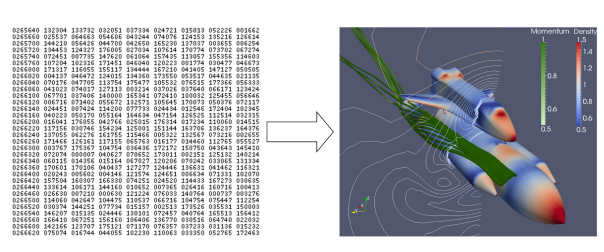
\includegraphics[width=0.5\textwidth]{images/Scient1.png} 
    \caption{Scientific Visualizzation}
    \label{fig:immagine}
\end{figure}
\textbf{1987}: La National Science Foundation degli Stati Uniti avvia "Visualizzazione nella computazione scientifica" come nuova disciplina, e un panel dell'ACM conia il termine "visualizzazione scientifica".
\begin{itemize}
    \item L'interesse è stato stimolato dall'aumento della potenza delle workstation degli scienziati, dai progressi negli algoritmi e dall'aumento delle dimensioni dei set di dati.
    \item La visualizzazione scientifica è definita come l'uso della grafica computerizzata per l'analisi e la presentazione di dati scientifici calcolati o misurati (Oxford English Dictionary, 1989).
    \item Nel 1990 si sono tenute le prime conferenze dedicate.
    \item Oggi è diventata una disciplina matura a sé stante.
\end{itemize}
Applicazioni nell'Ingegneria, Medicina, Scienza
Esempio:
La Tomografia Computerizzata (TC) a raggi X e la Risonanza Magnetica (RM) generano immagini (sezioni trasversali del paziente) che vengono combinate per produrre una rappresentazione volumetrica: da numeri a valori in scala di grigi.
Applicazioni nell'Ingegneria, Medicina, Scienza
Esempio: Dinamica dei fluidi computazionale (flusso d'aria, temperatura mappata a colori).
La Visualizzazione Scientifica riguarda anche la definizione di algoritmi efficienti per la manipolazione interattiva e l'esplorazione dei dati e delle loro caratteristiche.
\subsection{Basi di Scientific Visualization}
Nella Visualizzazione Scientifica, un dataset è dato da un oggetto geometrico di input (il dominio) su cui è definita una funzione, rappresentante gli attributi che desideriamo analizzare e visualizzare.
Le tecniche di visualizzazione dipendono dal tipo di dominio e dalla funzione. \\
$f : D \rightarrow A$ \\
\textbf{D} è il dominio, \textbf{A} è il dominio e $f$  è la funzione(attributi).
\subsubsection{Domain}
Dimensione (superfici 2D, volumi 3D), Discretizzazione, Geometria (incorporamento)
I dati sono rappresentati da un insieme finito di campioni. I dati sono estesi nello spazio tramite schemi di interpolazione. I dati hanno informazioni sulla posizione (incorporamento) e informazioni sulla connettività. 
Diverse discretizzazioni, in base all'incorporamento e alla connettività
Domini strutturati vs non strutturati, connettività fissa vs arbitraria.
\begin{figure}[H]
    \centering
    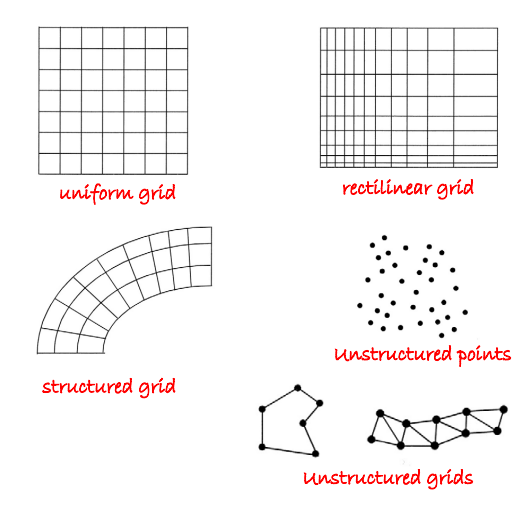
\includegraphics[width=0.5\textwidth]{images/DomDisk.png} 
    \caption{Domain discretization}
    \label{fig:immagine}
\end{figure}
\begin{itemize}
    \item \textbf{Griglie regolari uniformi}: anche chiamate "raster" (immagine a griglia 2D, volume a griglia 3D): tessellazioni del piano/spazio euclideo mediante elementi quadrati/cubici. I punti sono regolarmente spaziati lungo ciascuna direzione i-j-k, sistema di coordinate parallelo al sistema di coordinate globale x-y-z. Attributi collegati agli elementi della griglia. Rappresentazione semplice, ma "maledizione della dimensionalità".
    \item \textbf{Griglie rettilinee}: tessellazioni mediante rettangoli/cuboidi rettangolari (non necessariamente congruenti tra loro); griglie regolari, ma lo spaziamento dei punti lungo gli assi può variare. Utile per adattare il campionamento alla geometria dei dati. La connettività rimane fissa, ma è necessario conservare informazioni sullo spaziamento.
    \item \textbf{Griglia curvilinea}: stessa connettività delle griglie uniformi/rettilinee, ma geometria irregolare (i punti possono essere posizionati a coordinate arbitrarie - senza sovrapposizioni e auto-intersezioni).
    \item \textbf{Unstructured Points}: Nessuna informazione esplicita sulla connettività, geometria irregolare (chiamata anche nuvole di punti).
    \item \textbf{Unstructured Grids}: connettività e geometria irregolare, combinazioni differenti di celle permettono diverse scelte: triangoli e forme tetraedriche 
\end{itemize}
\subsubsection{Attributi}
Dimensione co-dominio (scalari, vettori, tensori)
Statico vs dipendente dal tipo (si applica solo agli attributi o sia al dominio che agli attributi)
Deterministico vs incerto (ad esempio, a causa del campionamento dello spazio dei parametri nelle simulazioni - osservazioni dell'insieme). La visualizzazione di dati incerti è un'area di ricerca a sé stante.
Gli attributi sono rappresentati da una funzione scalare.
\subsubsection{Transfer functions}
Come codificare i valori scalari?
Idea intuitiva: utilizzare una mappa dei colori attraverso un canale percettivo.
Disporre in modo continuo una tavolozza di colori e mapparla sulla retta reale.
\begin{figure}[H]
    \centering
    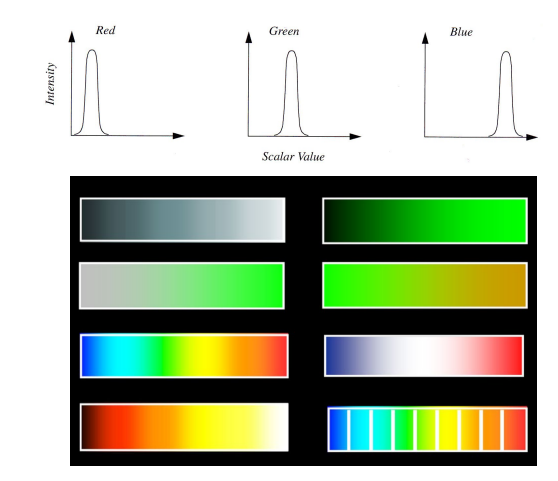
\includegraphics[width=0.5\textwidth]{images/transfFunctions.png} 
    \caption{Transfer functions}
    \label{fig:immagine}
\end{figure}
Per i volumi, le funzioni di trasferimento possono mappare gli scalari al colore e alla trasparenza. Le funzioni di trasferimento sono difficili da progettare. Esistono strumenti semi-automatici (gallerie di progettazione delle funzioni di trasferimento). Il conoscere il dominio di applicazione gioca un ruolo.
L'assegnazione di colore e trasparenza alla densità è anche conosciuta come classificazione.
\subsubsection{Volume Rendering}
Molte tecniche. L'idea alla base del "volume ray casting": ogni punto/cella dovrebbe contribuire; combinare le contribuzioni mediante integrazione.
\begin{figure}[H]
    \centering
    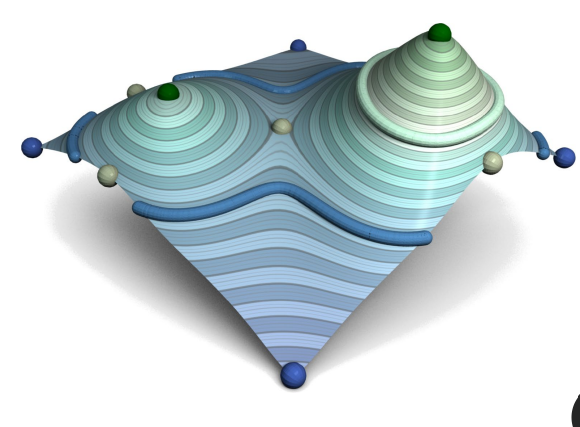
\includegraphics[width=0.5\textwidth]{images/ScalarField.png} 
    \caption{Scalar Field Visualization}
    \label{fig:immagine}
\end{figure}
Visualizzazione dei punti critici, delle isolinee e delle isosuperfici.Visualizzazione delle astrazioni topologiche
\subsubsection{Critical Points, continuous Case}
Nel contesto continuo, i punti critici sono punti di una varietà dove il gradiente di una funzione scalare continua si annulla.\\
Data Una funzione smmoth $f:M \rightarrowR$ Su una varietà liscia 𝑀, un punto P
\begin{figure}[H]
    \centering
    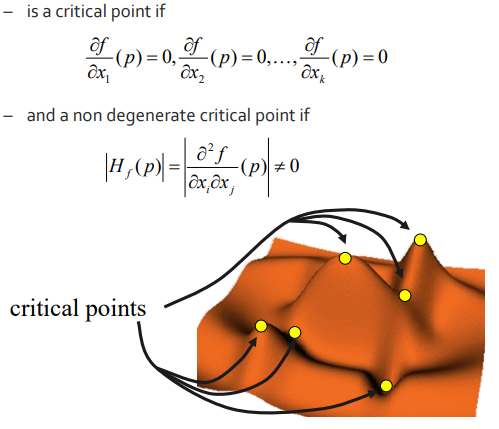
\includegraphics[width=0.8\textwidth]{images/CriticalPoints.png} 
    \caption{Critical Points}
    \label{fig:immagine}
\end{figure}
\subsubsection{Morse functions}
Una funzione liscia è chiamata Morse se tutti i suoi punti critici sono non degeneri.
\begin{itemize}
    \item Proprietà interessanti:
    \begin{itemize}
        \item Le funzioni di Morse sono un sottoinsieme denso di tutte le funzioni lisce.
        \item I punti critici sono isolati.
        \item Relazione tra i punti critici e la topologia della varietà.
    \end{itemize}
\end{itemize}
\subsubsection{Pice-wise linera (PL) settings}
Campo scalare PL: valori della funzione forniti sui vertici e interpolati ovunque altro utilizzando le coordinate baricentriche.
La nozione di punto critico si traduce direttamente dal contesto liscio a quello PL?
Svantaggio: il gradiente di un campo scalare PL è costante per pezzi (cioè costante all'interno di ciascun simplesso). Abbiamo bisogno di una definizione alternativa per i punti critici. Utilizziamo la connettività del link inferiore e superiore.
\begin{figure}[H]
    \centering
    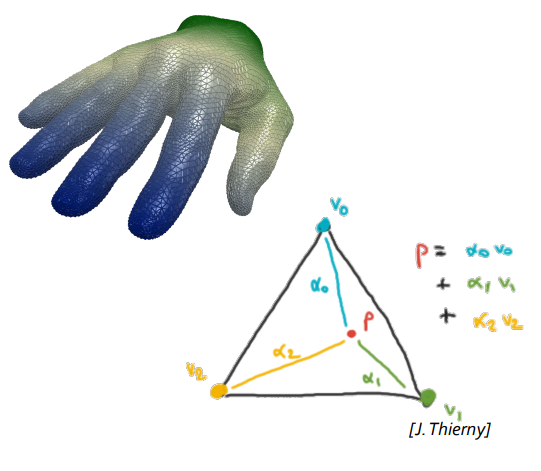
\includegraphics[width=0.8\textwidth]{images/Picewise.png} 
    \caption{Pice-wise liner setting}
    \label{fig:immagine}
\end{figure}
Il lower link LK-(v) (rispettivamente, l'upper link LK+(v)) di un vertice v relativo a un campo scalare PL f è il sottoinsieme del link di v tale che ciascuna delle sue 0-sottofacce abbia un valore f strettamente inferiore (rispettivamente, superiore) a v.

I vertici possono essere classificati come regolari o critici in base alla connettività del link superiore e inferiore. Un vertice v è regolare se sia il lower link LK-(v) che l'upper link LK+(v) sono semplicemente connessi. In caso contrario, v è un vertice critico e f(v) è un valore critico iso (in opposizione a un valore iso regolare).
Campo scalare PL
Valori critici distinti
Nessun punto critico degenerato
(in pratica: qualsiasi campo scalare PL dopo una perturbazione)
Problema: in pratica, i punti critici possono comparire in corrispondenza di lievi onde della funzione dovute al rumore nel processo di generazione dei dati (rumore di acquisizione, rumore numerico nella simulazione).
\begin{itemize}
    \item Per rendere i punti critici affidabili e utili nella pratica, è necessario un meccanismo per classificare i punti critici come rumore o segnale.
    \item Possiamo utilizzare l'Omelogia Persistente.
\end{itemize}

\subsection{Filtration}
\subsection{Reeb graph}